%************************************************
\chapter{Introducción}\label{ch:introduction}
%************************************************

En la actualidad, para demostrar que conocemos un secreto a alguien, utilizamos un medio donde nadie nos espíe y le contamos el secreto directamente a nuestro interlocutor. En el ámbito de la criptografía, cifraríamos el secreto con una clave, simétrica o asimétrica, tal que, sólo quien conozca la clave de descifrado pueda leer nuestro secreto. Esto es la base de las comunicaciones seguras en Internet. Ciframos nuestra contraseña de modo que sólo el servidor de correo pueda leerla, pudiendo iniciar nuestra sesión sin que ningún espía nos la pueda robar. El problema es que hay dos partes que conocen el secreto, dos puntos de ataque.

Existe un área de la criptología que se encarga de abordar este problema, demostrar que conocemos algo, pero sin que de la misma prueba se obtenga más información. Estos métodos se conocen como pruebas de conocimiento cero. Elegimos estudiar estas técnicas a raíz del TFG de Ing. Informática, \textit{Integración de Idemix en entornos IoT}, donde Idemix es un protocolo criptográfico basado en pruebas de conocimiento cero. En la Facultad de Informática no habría sido posible un estudio en profundidad como el que presentamos aquí, por ello, ese trabajo lo limitamos a la implementación, mientras que con este conseguiremos entender por qué funciona realmente.

Para ilustrar las pruebas de conocimiento cero, en 1990, Guillou, Quisquater y Berson publicaron en \textit{How to Explain Zero-Knowledge Protocols to Your Children} \citep{ZKPcave:story} una historia sobre cómo Alí Babá demostró poder abrir la cueva sin decir a nadie cuáles eran las palabras mágicas. Aquí presentamos una versión resumida que destaca las propiedades básicas de estos métodos:

\hfil

\begin{quote}
Imaginemos una cueva, donde el camino principal se bifurca y al final de cada pasillo los caminos se vuelven a encontrar, formando una especie de anillo. En el punto en que se unen, dentro de la cueva, hay una puerta mágica con una palabra secreta, la cual permite abrirla y cruzar al otro lado.

\textbf{P}aula conoce la clave secreta y quiere \textbf{p}robarlo a su amigo Víctor, pero sin tener que revelársela. Paula y Víctor quedan en la entrada de la cueva con unos \textit{walkie-talkies}, de modo que Víctor esperará fuera y Paula entrará a la cueva y tomará uno de los pasillos, que llamaremos A y B, sin decirle cuál a Víctor.


Al llegar a la puerta, Paula avisa a Víctor para que entre a la cueva y espere en la bifurcación, donde \textbf{V}íctor, para intentar \textbf{v}erificar que Paula conoce la palabra secreta, le indicará por qué pasillo quiere que vuelva, el A o el B.


Si Paula realmente conoce el secreto, podrá volver a la bifurcación por el pasillo solicitado, abriendo, si es preciso, la puerta.

Pero en caso de no conocer la clave, al entrar por uno de los pasillos, tenía una probabilidad del $50\%$ de adivinar cuál pediría Víctor.

Víctor no se queda contento con una sola prueba, pues Paula podría haber tenido suerte, así que la repiten hasta que se convence. Con unas 20 repeticiones, Paula tendría solo una probabilidad de $2^{-20}$, prácticamente nula, de acertar todas las veces y engañar así a Víctor.

\textbf{E}va, curiosa de qué hacían Víctor y Paula en la cueva, \textbf{e}spía a Víctor durante todo el proceso. Eva no sabe si Paula y Víctor han acordado previamente qué pasillo pedir por el \textit{walkie-talkie}, y sólo Víctor está seguro de que él los estaba eligiendo al azar y sin previo acuerdo.%, por eso, Eva no puede estar segura de si Paula conoce la clave secreta, o bien estaban \textbf{s}imulando todo para engañarla por cotilla.

Más tarde Eva habla con Víctor, que está seguro de que Paula conoce la clave, y éste querría convencer también a Eva, pero como él no conoce la clave, no puede repetir la prueba a Eva, sólo Paula puede realizarla con éxito.
\end{quote}



\begin{figure}[!htb]
	\minipage{0.3\textwidth}
	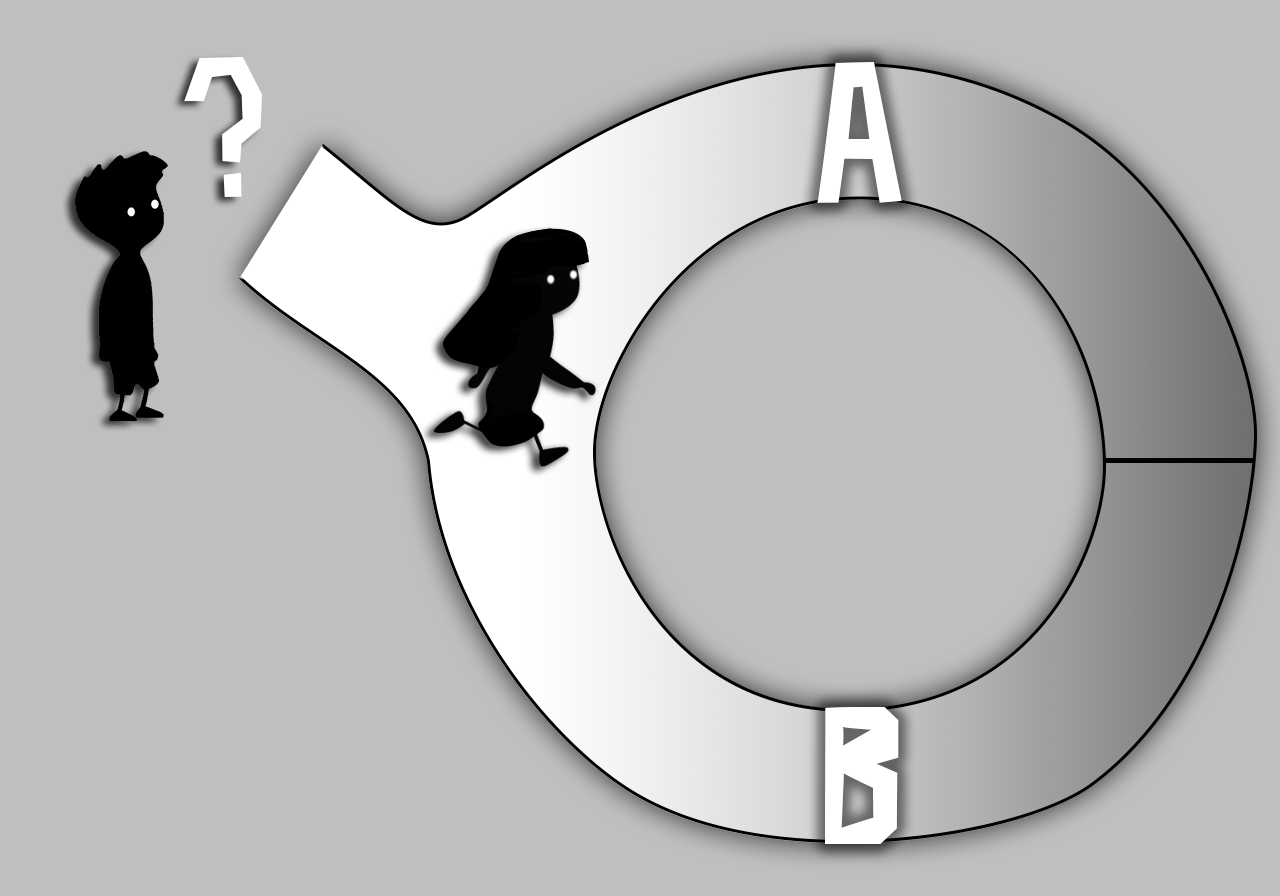
\includegraphics[width=\linewidth]{gfx/graficoJL_ZKP_1}
	\caption*{La cueva \citep{ZKPcave:fig}. Paula entra por A o B al azar. Víctor espera fuera.}\label{fig:awesome_image1}
	\endminipage\hfill
	\minipage{0.3\textwidth}
	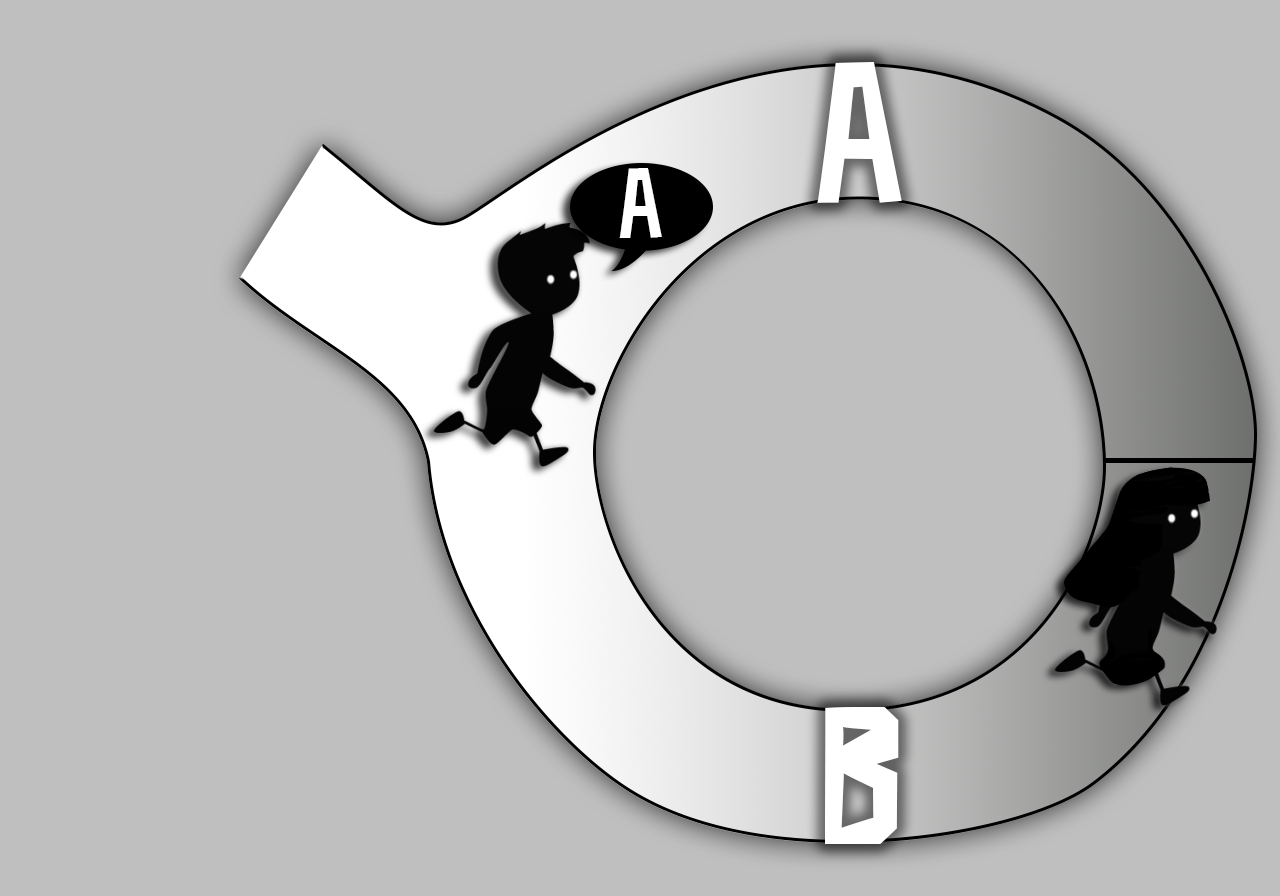
\includegraphics[width=\linewidth]{gfx/graficoJL_ZKP_2}
	\caption*{Víctor elige al azar por dónde quiere que regrese Paula.}\label{fig:awesome_image2}
	\endminipage\hfill
	\minipage{0.3\textwidth}%
	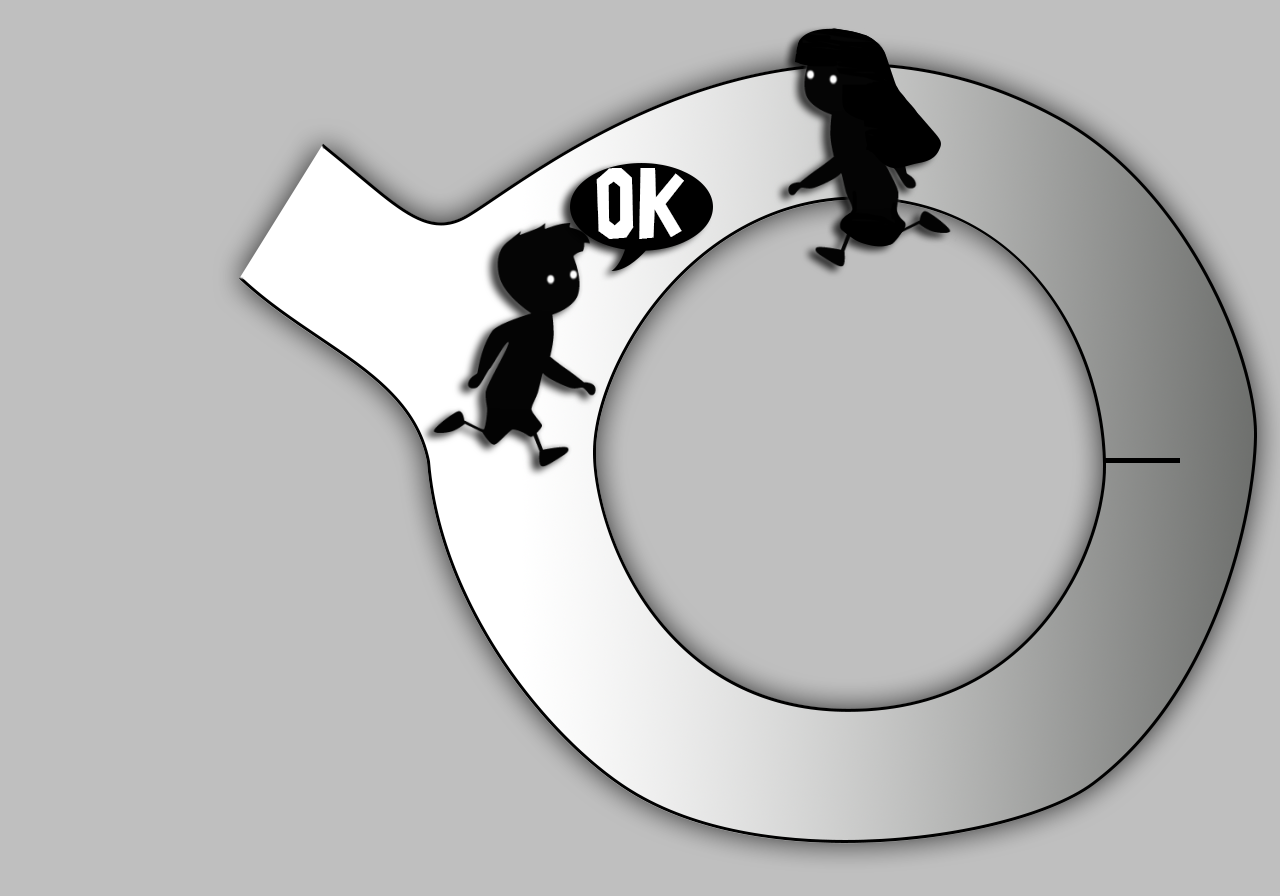
\includegraphics[width=\linewidth]{gfx/graficoJL_ZKP_3}
	\caption*{Paula vuelve por el camino pedido.\\ }\label{fig:awesome_image3}
	\endminipage
\end{figure}



\hfil

En el estudio formal de las Pruebas de Conocimiento Cero se utilizan distintos tipos de problemas, y los más utilizados est\'an relacionados con la \textbf{teor\'ia de n\'umeros}
y la \textbf{teor\'ia de grafos}. Son problemas difíciles de resolver para quien no conoce alguna información extra de los mismos, que en nuestra fábula serían el problema de abrir la puerta sin conocer la
palabra mágica. Los problemas más representativos de las Pruebas de Conocimiento Cero son el del logaritmo discreto, la raíz cuadrada modular, el isomorfismo de grafos, el c\'alculo de caminos
hamiltonianos en grafos y la 3-coloración de grafos.

La memoria se divide en tres partes, en la primera parte estudiaremos todos estos problemas, empezando por
definir qué se entiende por un problema \textit{difícil} desde el punto de vista de la computaci\'on, para despu\'es describir formalmente los problemas mencionados anteriormente
as\'i como los algoritmos que nos permiten resolverlos cuando disponemos de una informaci\'on adicional (el secreto).

La segunda parte de la memoria se dedicar\'a a las Pruebas de Conocimiento Cero en s\'i mismas, definiremos qué propiedades debe cumplir una prueba de este tipo,
enunciaremos pruebas que utilicen los problemas anteriores, y demostraremos que cada una de ellas cumple la definición.

La tercera parte de la memoria estar\'a dedicada a las aplicaciones prácticas de estas Pruebas de Conocimiento Cero. La utilizaci\'on de estos algoritmos permite resolver problemas
relacionados con la privacidad de las comunicaciones, aumentando la seguridad y la funcionalidad de las aplicaciones.

Por \'ultimo, dedicaremos un ap\'endice a mostrar algunas implementaciones de estos algoritmos utilizando {\tt sage}, que es un software matem\'atico basado en Python de
libre distribuci\'on.
